\chapter{Einleitung}

Softwarequalitätsmanagement (SQM) ist ein entscheidender Aspekt bei der Entwicklung und Implementierung von Softwarelösungen, 
um sicherzustellen, dass sie effizient, sicher und zuverlässig sind. In dieser Hausarbeit werden wir uns mit dem Vorgehen 
hinsichtlich SQM auseinandersetzen und Optimierungen entwerfen, indem wir ein praktisches Fallbeispiel untersuchen. 
Unser Anwendungsbeispiel ist die Entwicklung einer firmeninternen Lernplattform mit Gamification. 
Dieses Beispiel dient dazu, sowohl theoretisches Wissen als auch praktische 
Anwendungsfähigkeiten in Bezug auf SQM nachzuweisen.

\begin{figure}
	\centering
	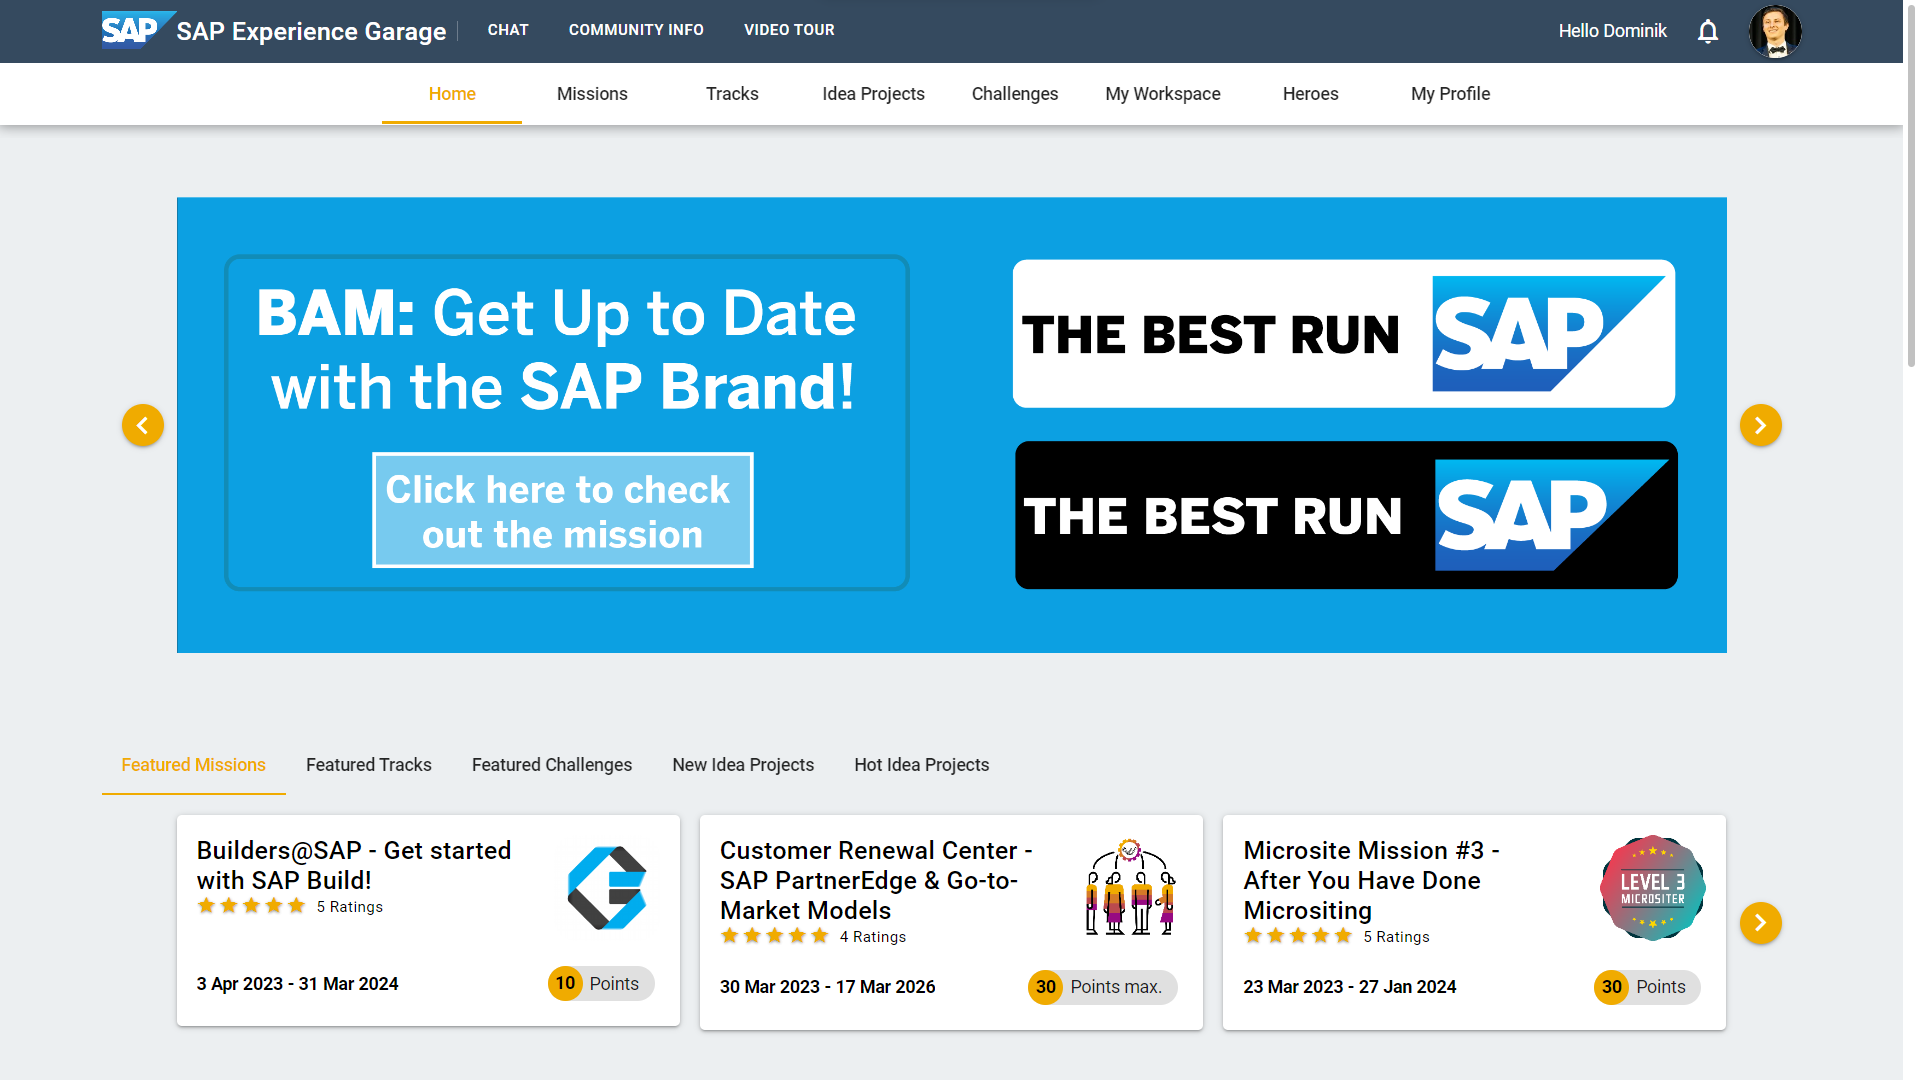
\includegraphics[width=1.\textwidth]{Bilder/dh-website.png} 
	\caption{Die Abbildung zeigt die Landing-Page der Digital-Heroes-Lernplattform. 
    Insbesondere lässt sich der Tab der \textit{Featured Missions} erkennen.}
	\label{fig:dh-website}
\end{figure} 

Bei meiner Firma, der SAP, gibt es intern eine Lernplattform die Gamification nutzt, um SAP-interne Prozesse 
spielerisch den Kollegen zu vermitteln. Diese Plattform heißt \textit{Digital Heroes}. 
Bisher können die Kollegen die Lernplattform nach konkreten Inhalten durchsuchen. 
Außerdem können die Moderatoren bestimmte Inhalte auf der Startseite featuren. Es gibt jedoch keine 
personalisierten Empfehlungen von Lerninhalten für die Nutzer der Plattform. 
\autoref{fig:dh-website} zeigt die Landing-Page der Lernplattform. \\
Ich bin in die Abteilung, um eine in-house Recommendation Engine (RE) zu integrieren, die den Nutzern Inhalte vorschlagen soll. 
Jedoch besteht die Abteilung zum Großteil aus Studenten, wobei alle Entwickler Studenten sind. 
Die Lernplattform ist als Studentenprojekt entstanden. 
Die technischen Komponenten, sowie die Prozesse sind in keinem Zustand, um weitere Features hinzuzufügen.
Bevor ich also die Integration der neuen Softwarekomponente durchführen kann, 
müssen einige grundlegende Änderungen durchgeführt, oder zumindest auf den Weg gebracht werden.
Die Verbesserung der bestehenden Codequalität und Entwicklungsprozesse wird Ziel dieser Arbeit sein.

Um dieses Ziel zu erreichen, soll das erworbene Wissen aus der Softwarequalität-Vorlesung genutzt werden, 
um das Problem kritisch zu analysieren und zu optimieren. 
Dafür wird zunächst die Applikation und deren Architektur beschrieben, 
dann die Ist-Situation der Codequalität und der Entwicklungsprozesse untersucht, 
wobei betrachtet wird, warum die Zustände nicht länger tragbar sind. 
Daraufhin werden die Gründe erörtert, die zu diesem Zustand geführt haben, 
sodass nachhaltige Lösungsstrategien entwickelt werden können 
und schließlich wird erörtert, wie 
die Soll-Situation aussehen sollte und wie diese erreicht werden kann. 
Für die Optimierungen werden die Inhalte aus der SQM-Vorlesung herangezogen. 
Abschließend werden in einer Zusammenfassung die grundlegenden Erkenntnisse und Verbesserungen nochmals bündig dargelegt.



